% Top-level schematic of the structural Booth multiplier (non-behavioural path).
% Build:  pdflatex schematic.tex
\documentclass[border=8pt]{standalone}
\usepackage{tikz}
\usepackage{amsmath}
\usetikzlibrary{arrows.meta,positioning,fit,backgrounds,calc}

\definecolor{cReg}{HTML}{888780}   \definecolor{cRegBg}{HTML}{F1EFE8}
\definecolor{cEnc}{HTML}{0F6E56}   \definecolor{cEncBg}{HTML}{E1F5EE}
\definecolor{cMux}{HTML}{534AB7}   \definecolor{cMuxBg}{HTML}{EEEDFE}
\definecolor{cCor}{HTML}{993C1D}   \definecolor{cCorBg}{HTML}{FAECE7}
\definecolor{cTree}{HTML}{3B6D11}  \definecolor{cTreeBg}{HTML}{EAF3DE}
\definecolor{cAdd}{HTML}{185FA5}   \definecolor{cAddBg}{HTML}{E6F1FB}
\definecolor{cWire}{HTML}{5F5E5A}

\begin{document}
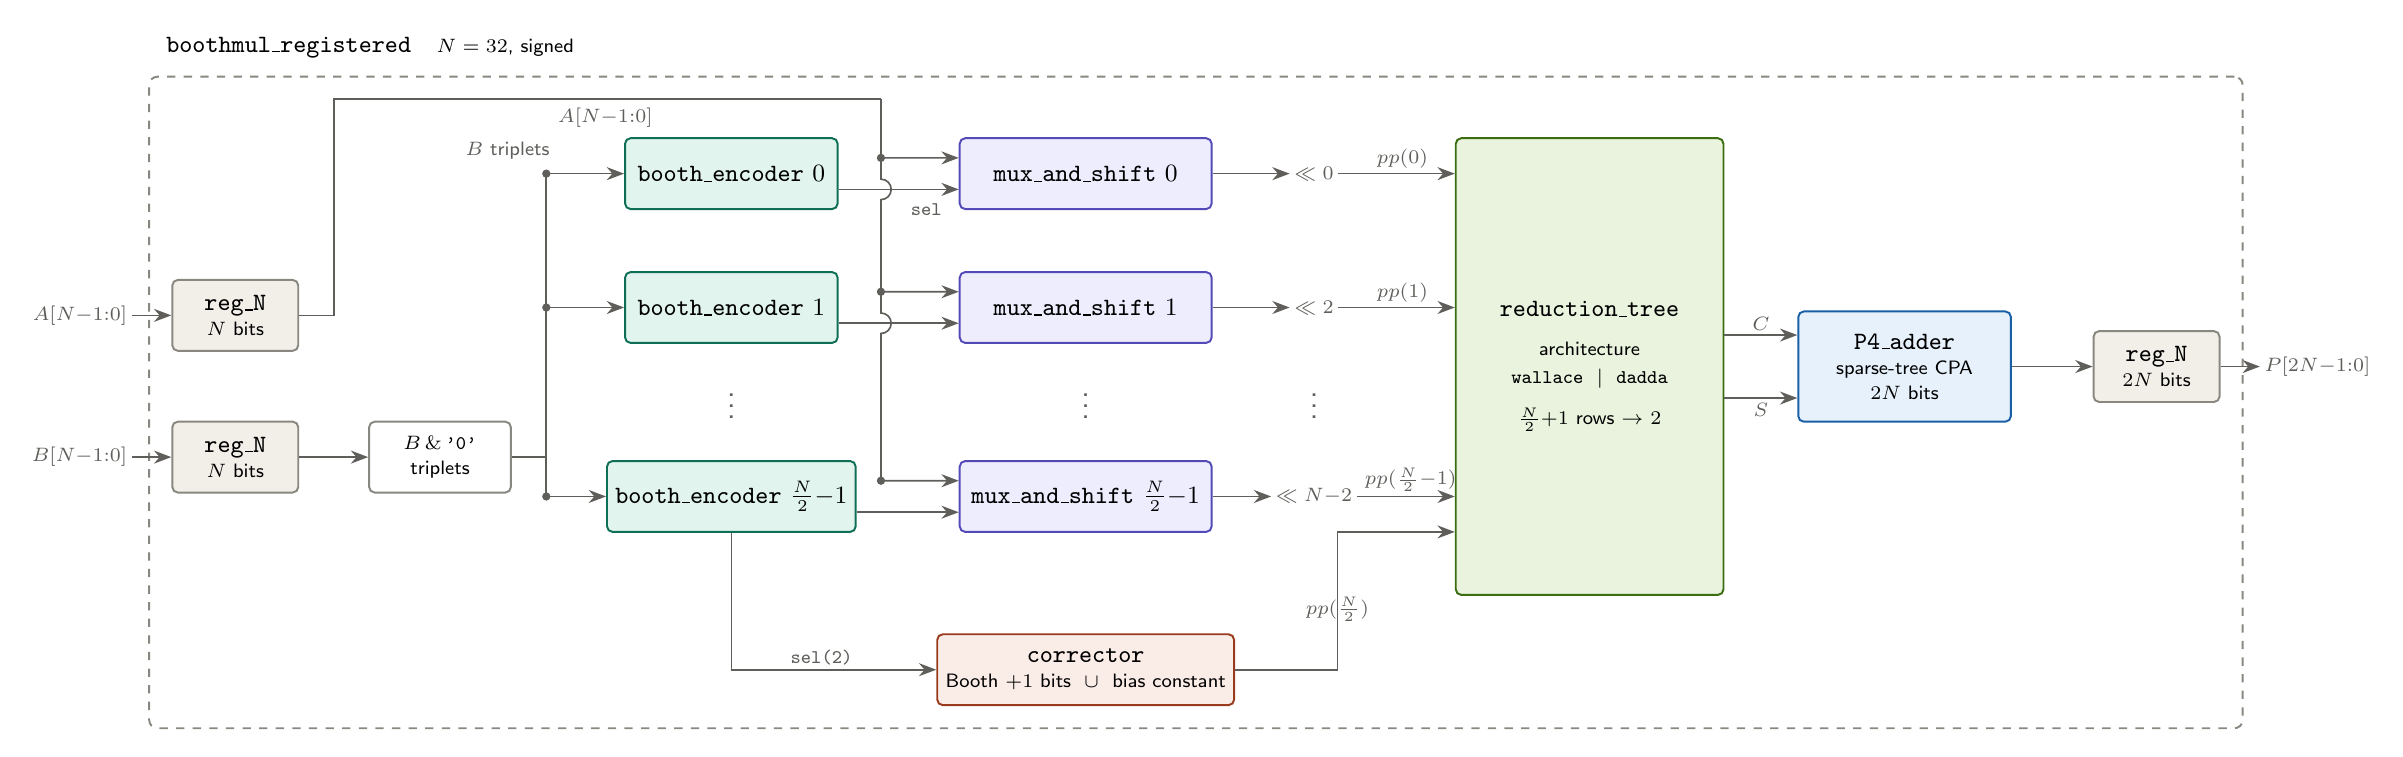
\begin{tikzpicture}[
  font=\sffamily\small,
  blk/.style={rectangle, rounded corners=2pt, draw, line width=0.7pt,
              minimum height=9mm, align=center, inner sep=3pt},
  reg/.style ={blk, draw=cReg,  fill=cRegBg,  minimum width=16mm},
  enc/.style ={blk, draw=cEnc,  fill=cEncBg,  minimum width=27mm},
  mux/.style ={blk, draw=cMux,  fill=cMuxBg,  minimum width=32mm},
  cor/.style ={blk, draw=cCor,  fill=cCorBg,  minimum width=36mm},
  tree/.style={blk, draw=cTree, fill=cTreeBg, minimum width=34mm},
  add/.style ={blk, draw=cAdd,  fill=cAddBg,  minimum width=27mm},
  w/.style  ={-{Stealth[length=2.2mm]}, draw=cWire, line width=0.6pt},
  bus/.style={draw=cWire, line width=0.6pt},
  lbl/.style={font=\sffamily\scriptsize, text=cWire, inner sep=1.5pt},
  dots/.style={font=\sffamily\large, text=cWire}
]

% ------------------------------------------------------------- coordinates
\def\xreg{0}    \def\xtrip{2.6}  \def\xtbus{3.95}
\def\xenc{6.3}  \def\xabus{8.2}  \def\xmux{10.8}
\def\xsh{13.7}  \def\xtree{17.2} \def\xadd{21.2}  \def\xpreg{24.4}
\def\yA{3.2}    \def\yB{1.5}     \def\yC{-0.9}

% --------------------------------------------------------------- registers
\node[reg] (areg) at (\xreg,  1.4) {\texttt{reg\_N}\\[-2pt]\scriptsize $N$ bits};
\node[reg] (breg) at (\xreg, -0.4) {\texttt{reg\_N}\\[-2pt]\scriptsize $N$ bits};
\node[lbl, left=5mm of areg] (Ain) {$A[N{-}1{:}0]$};
\node[lbl, left=5mm of breg] (Bin) {$B[N{-}1{:}0]$};
\draw[w] (Ain) -- (areg);   \draw[w] (Bin) -- (breg);

% -------------------------------------------------------- triplet slicing
\node[blk, draw=cReg, fill=white, minimum width=18mm] (trip) at (\xtrip,-0.4)
     {\scriptsize $B\,\&\,\texttt{'0'}$\\[-2pt]\scriptsize triplets};
\draw[w] (breg) -- (trip);

% -------------------------------------------------------------- the stages
\node[enc] (e0) at (\xenc, \yA) {\texttt{booth\_encoder} $0$};
\node[enc] (e1) at (\xenc, \yB) {\texttt{booth\_encoder} $1$};
\node[dots]      at (\xenc, 0.35) {$\vdots$};
\node[enc] (ek) at (\xenc, \yC) {\texttt{booth\_encoder} $\tfrac{N}{2}{-}1$};

\node[mux] (m0) at (\xmux, \yA) {\texttt{mux\_and\_shift} $0$};
\node[mux] (m1) at (\xmux, \yB) {\texttt{mux\_and\_shift} $1$};
\node[dots]      at (\xmux, 0.35) {$\vdots$};
\node[mux] (mk) at (\xmux, \yC) {\texttt{mux\_and\_shift} $\tfrac{N}{2}{-}1$};

% triplet bus: vertical spine, then one arrow per encoder
\draw[bus] (trip.east) -- (\xtbus,-0.4);
\draw[bus] (\xtbus,\yC) -- (\xtbus,\yA);
\foreach \n/\yy in {e0/\yA, e1/\yB, ek/\yC}{
  \draw[w] (\xtbus,\yy) -- (\n.west);
  \fill[cWire] (\xtbus,\yy) circle (1.5pt);}
\node[lbl, anchor=south east] at (\xtbus+0.10,\yA+0.12) {$B$ triplets};

% A bus: up over the top of the encoder column, across, then down a spine
% between the encoders and the muxes, so it never runs over a block.
% The spine stops at the lowest tap point; where it meets a sel wire it hops
% over with a small semicircle, and every tap is marked with a junction dot.
\def\yover{4.15}
\def\hop{0.13}
\coordinate (abusL) at (1.25,\yover);  \coordinate (abusR) at (\xabus,\yover);
\draw[bus] (areg.east) -- (1.25,1.4) -- (abusL) -- (abusR);

% sel, entering each mux slightly below centre (drawn first, the A bus hops it)
\foreach \e/\m in {e0/m0, e1/m1, ek/mk}{
  \draw[w] ([yshift=-2mm]\e.east) -- ([yshift=-2mm]\m.west);}
\node[lbl, anchor=west] at (8.52,\yA-0.46) {\texttt{sel}};

% the vertical spine, hopping over the sel wires at yA-0.2 and yB-0.2
\draw[bus] (\xabus,\yover) -- (\xabus,\yA-0.2+\hop)
           arc[start angle=90, end angle=-90, radius=\hop]
        -- (\xabus,\yB-0.2+\hop)
           arc[start angle=90, end angle=-90, radius=\hop]
        -- (\xabus,\yC+0.2);
\node[lbl, anchor=north] at (4.7,\yover-0.06) {$A[N{-}1{:}0]$};

% taps into the muxes, each marked with a junction dot
\foreach \n/\yy in {m0/\yA, m1/\yB, mk/\yC}{
  \draw[w] (\xabus,\yy+0.2) -- ([yshift=2mm]\n.west);
  \fill[cWire] (\xabus,\yy+0.2) circle (1.5pt);}

% ---------------------------------------------------------------- corrector
\node[cor] (cor) at (\xmux, -3.1)
  {\texttt{corrector}\\[-2pt]\scriptsize Booth $+1$ bits $\;\cup\;$ bias constant};
\draw[w] (ek.south) |- node[lbl, pos=0.72, above]{\texttt{sel(2)}} (cor.west);

% ------------------------------------------------------- weighting by $4^i$
\node[lbl] (s0) at (\xsh, \yA) {$\ll 0$};
\node[lbl] (s1) at (\xsh, \yB) {$\ll 2$};
\node[dots]     at (\xsh, 0.35) {$\vdots$};
\node[lbl] (sk) at (\xsh, \yC) {$\ll N{-}2$};
\draw[w] (m0) -- (s0);  \draw[w] (m1) -- (s1);  \draw[w] (mk) -- (sk);

% ----------------------------------------------------------- reduction tree
\node[tree, minimum height=58mm] (tree) at (\xtree, 0.75)
  {\texttt{reduction\_tree}\\[3pt]
   \scriptsize architecture\\[-1pt]\scriptsize \texttt{wallace} $\;|\;$ \texttt{dadda}\\[4pt]
   \scriptsize $\tfrac{N}{2}{+}1$ rows $\rightarrow$ $2$};

\foreach \n/\t in {s0/{$pp(0)$}, s1/{$pp(1)$}, sk/{$pp(\tfrac{N}{2}{-}1)$}}{
  \draw[w] (\n) -- node[lbl, above, pos=0.55]{\t} (\n-|tree.west);}
\draw[w] (cor.east) -- ++(1.3,0) |- node[lbl, pos=0.28, below]{$pp(\tfrac{N}{2})$}
      ([yshift=-21mm]tree.west);

% ------------------------------------------------------------- final adder
\node[add, minimum height=14mm] (p4) at (\xadd, 0.75)
  {\texttt{P4\_adder}\\[-2pt]\scriptsize sparse-tree CPA\\[-2pt]\scriptsize $2N$ bits};
\draw[w] ([yshift=4mm]tree.east) -- node[lbl,above]{$C$} ([yshift=4mm]p4.west);
\draw[w] ([yshift=-4mm]tree.east) -- node[lbl,below]{$S$} ([yshift=-4mm]p4.west);

% ------------------------------------------------------------- output reg
\node[reg] (preg) at (\xpreg, 0.75) {\texttt{reg\_N}\\[-2pt]\scriptsize $2N$ bits};
\draw[w] (p4) -- (preg);
\node[lbl, right=5mm of preg] (Pout) {$P[2N{-}1{:}0]$};
\draw[w] (preg) -- (Pout);

% ------------------------------------------------------------- boundary box
\begin{scope}[on background layer]
  \node[draw=cReg, line width=0.7pt, rounded corners=3pt, dashed,
        fit=(areg)(breg)(e0)(cor)(tree)(p4)(preg)(abusL)(abusR), inner sep=8pt] (top) {};
\end{scope}
\node[anchor=south west, font=\sffamily\small] at ($(top.north west)+(3pt,3pt)$)
  {\texttt{\textbf{boothmul\_registered}}\quad\scriptsize $N=32$, signed};

\end{tikzpicture}
\end{document}
